%%poster03.tex with figures in TikZ
\documentclass[36pt]{sciposter}
\usepackage{preposterTikz} %package with the preamble.
\usepackage{fourier} 
    \usepackage{caption} 
\usepackage{array}
\usepackage{tabularx} % for 'tabularx' environment
\usepackage{graphicx} % 그래픽을 위한 패키지
\usepackage{xcolor}
\usepackage{amsmath}
\usepackage{amsfonts}
\usepackage{latexsym,amsmath,xcolor,multicol,booktabs,calligra}
\usepackage{graphicx,pstricks,listings,stackengine}
\usepackage{subcaption}
\usepackage{graphicx}
\usepackage{subcaption}
\usepackage{amsfonts}
\usepackage{amsmath}
\usepackage{multirow}
\usepackage{algorithm}
\usepackage{algpseudocode}
\usepackage{varwidth}
\usepackage{adjustbox}
\usepackage{amsthm}
\usepackage{amssymb}
\usepackage{mathrsfs}
\usepackage{graphicx}
\usepackage{adjustbox}
\usepackage{enumitem}




\geometry{paperwidth=90cm,paperheight=100cm,centering,textwidth=85cm,textheight=94cm,left=0cm,top=2cm}
\pgfplotsset{compat=1.18}
%**********************************************
% Colors
\definecolor{col_CN}{HTML}{2215EA}
\definecolor{col_MCI}{HTML}{15EA3C}
\definecolor{col_AD}{HTML}{EA1515}


%==================================
\captionsetup[figure]{labelformat=empty} % figure 캡션의 라벨 포맷을 비움



%**********************************************
\begin{document}

\onehalfspacing

%%Fill in the commands below with your details.
\newcommand{\tituloposter}{Functional Data Analysis Approach on Functional Connectivity from}%%title of the poster
\newcommand{\titulogrande}{Resting-State fMRI for Classification of Dementia Patients} 

%%Fill in WITHIN THE parenthesis only if the title does not fit on one line.
%%ATTENTION: If you are not going to use the second line, just do not write anything between "{}".

% \newcommand{\nome}{Ido Ji$^{(a)}$, first name1, LAST NAME 2$^{(b)}$, first name2, LAST NAME 3$^{(b)}$, first name3} %%your name

\newcommand{\nome}{Ido Ji$^{(a)}$, Eunjee Lee$^{(b)}$} %%your name
\newcommand{\instituicao}{$(a)$ Department of Bio AI Convergence, Chungnam National University, $(b)$. Department of Information Statistics, Chungnam National University} %%institution

%%title made with TikZ (using \newcommand).
% \titulo{sifsc}{WhiteSquare}{BoxCol} %blue
%Place the SIICUSP logo instead of the white square


% 타이틀 기준 왼쪽 로고 : WhiteSquare (아무것도 안 넣는 경우)
% 타이틀 기준 오른쪽 로고 : CNU
\titulo{WhiteSquare}{CNU.png}{BoxCol} %blue


%%title made with TikZ (using \newcommand).
% \titulo{sifsc}{
%     
\includegraphics[width=1cm]{Figures/ci_simbol_v2.png} % 이미지 크기 및 파일명 조정
% }{BoxCol} %blue

    

\vspace{4cm} %space



%=======================================
% Abstract
%=======================================
% \section*{\tituloA{Abstract}}


Lorem ipsum dolor sit amet, consectetur adipiscing elit. Aliquam porta justo vel vehicula cursus. Quisque porta lectus sit amet mattis accumsan. Donec nulla leo, vestibulum quis suscipit eu, porta vel tellus. Phasellus sed pellentesque mauris. Mauris posuere massa magna, at gravida nibh dapibus nec. Curabitur non nibh non tortor elementum hendrerit id id risus. 



\begin{multicols}{2}
%%Paragraph.
\setlength{\parindent}{3em}


%=======================================
\section*{\tituloA{1.Motivation}}



\begin{tikzfigure}
    \centering
    \begin{minipage}{.32\linewidth}
      \centering
      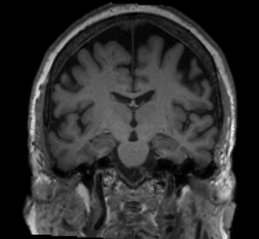
\includegraphics[height=6cm]{Figures/Brain__1.CN.png}
      \captionof{figure}{Normal}
    \end{minipage}%
    \hfill
    %================================
    \begin{minipage}{.32\linewidth}
      \centering
      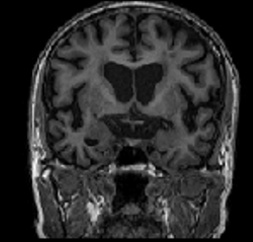
\includegraphics[height=6cm]{Figures/Brain__3.AD.png}
      \captionof{figure}{Alzheimer's Disease}
    \end{minipage}
    \hfill
    %================================
    \begin{minipage}{.32\linewidth}
      \centering
      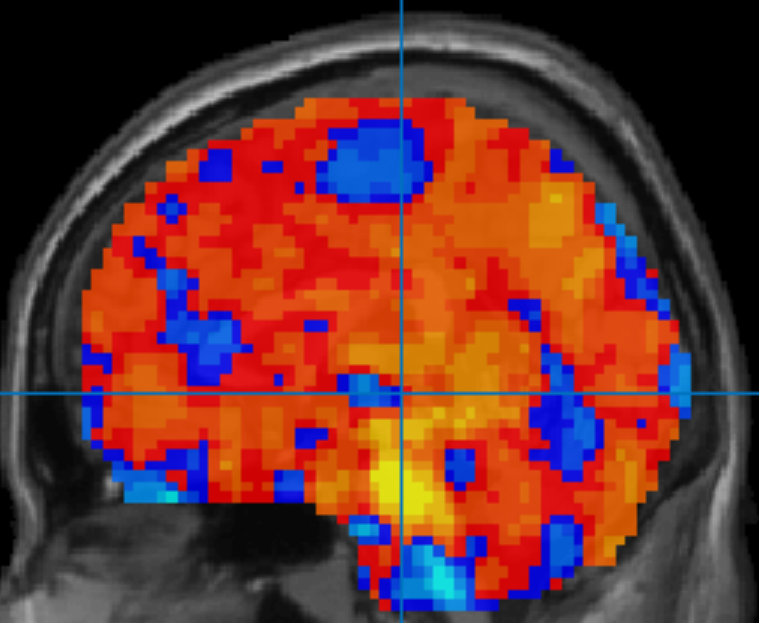
\includegraphics[height=6cm]{Figures/FC_Sagittal.png}
      \captionof{figure}{Functional Activity}
    \end{minipage}
\end{tikzfigure}




    
  %   \begin{tikzfigure}
  %       \centering
  %       \begin{minipage}{.50\linewidth}
  %         \centering
  %         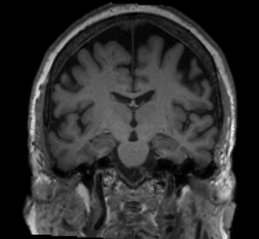
\includegraphics[height=9cm]{Figures/Brain__1.CN.png}
  %         \caption{\textcolor{col_CN}{CN}}
  %       \end{minipage}%
  %       \hfill
  %       \begin{minipage}{.50\linewidth}
  %         \centering
  %         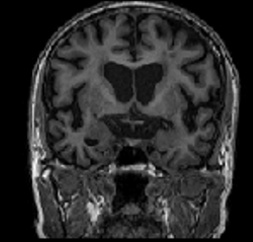
\includegraphics[height=9cm]{Figures/Brain__3.AD.png}
  %         \caption{\textcolor{col_AD}{Dementia}}
  %       \end{minipage}
  %   \end{tikzfigure}
    
    \begin{itemize}
        % \item Dementia shows 3 progressive stages.     
        \item \small Alzheimer's Disease (AD) is incurable.

        \item \small  Different \textbf{brain atrophy} can be seen between AD and normal patients.

        \item \small  By monitoring and identifying related brain regions that are characteristic of AD, researchers can better understand the progression of the disease, leading to the development of more effective interventions.
        
        \item \small  Hence, their \textbf{functional activity} in Resting-State fMRI (RS-fMRI) should be different. 

        \item \small From RS-fMRI, we can obtain \textbf{blood-oxygen-level-dependent (BOLD) times courses} for each region of interest (ROI) on brains.

    \end{itemize}
% \noindent

%=======================================
\section*{\tituloA{2.Functional Data Analysis}}

   \centering 
   \begin{figure}[ht]
    \centering
    \begin{minipage}{0.24\linewidth}
        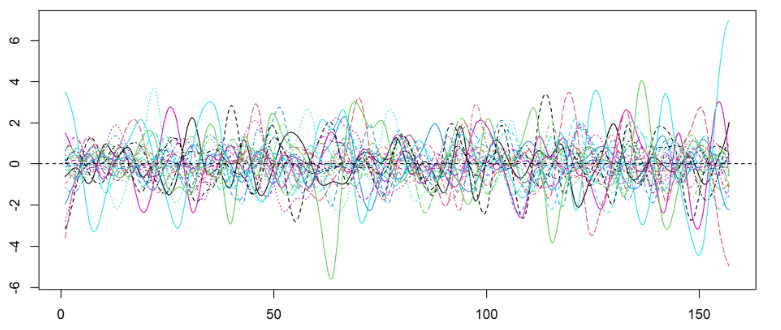
\includegraphics[width=\linewidth]{Figures/After_expansion.png}
         \captionsetup{font=small} % 캡션의 글자 크기를 작게 설정
         \captionof{figure}{BOLD Signals}
    \end{minipage}
    \hfill
    \begin{minipage}{0.14\linewidth}
        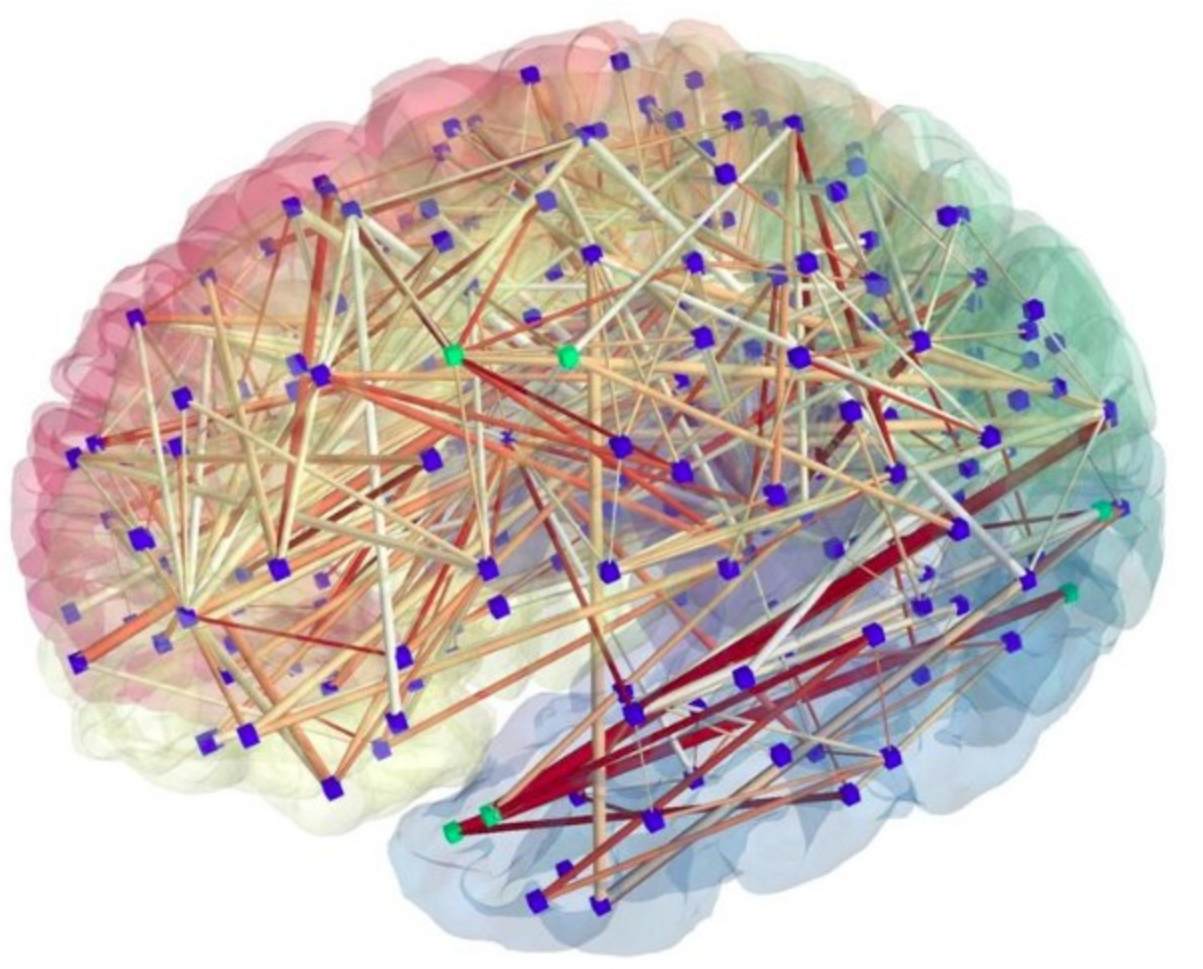
\includegraphics[width=\linewidth]{Figures/Functional Connectivity.png}
        \captionsetup{font=small} % 캡션의 글자 크기를 작게 설정
         \captionof{figure}{FC}
        \label{fig:image2}
    \end{minipage}
    \hfill
    \begin{minipage}{0.20\linewidth}
        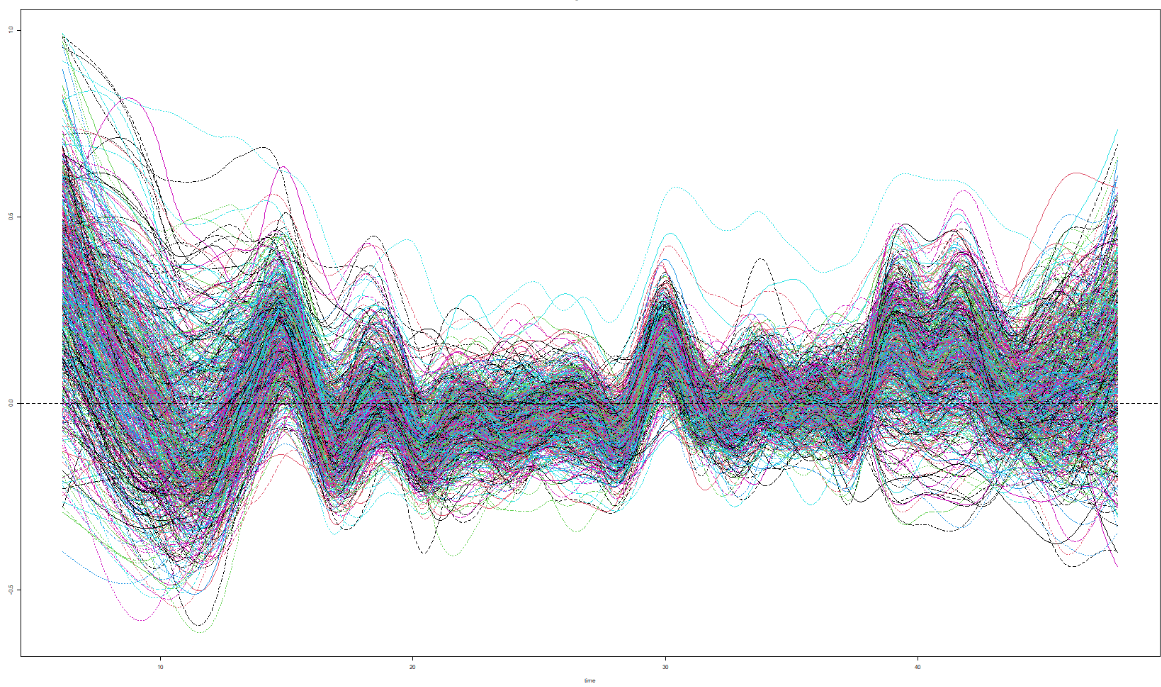
\includegraphics[width=\linewidth]{Figures/FC___FunImgARglobalCWSF___Smoothing.png}
        \captionsetup{font=small} % 캡션의 글자 크기를 작게 설정
         \captionof{figure}{Smoothed FC}
        \label{fig:image3}
    \end{minipage}
    \hfill
    \begin{minipage}{0.38\linewidth}
        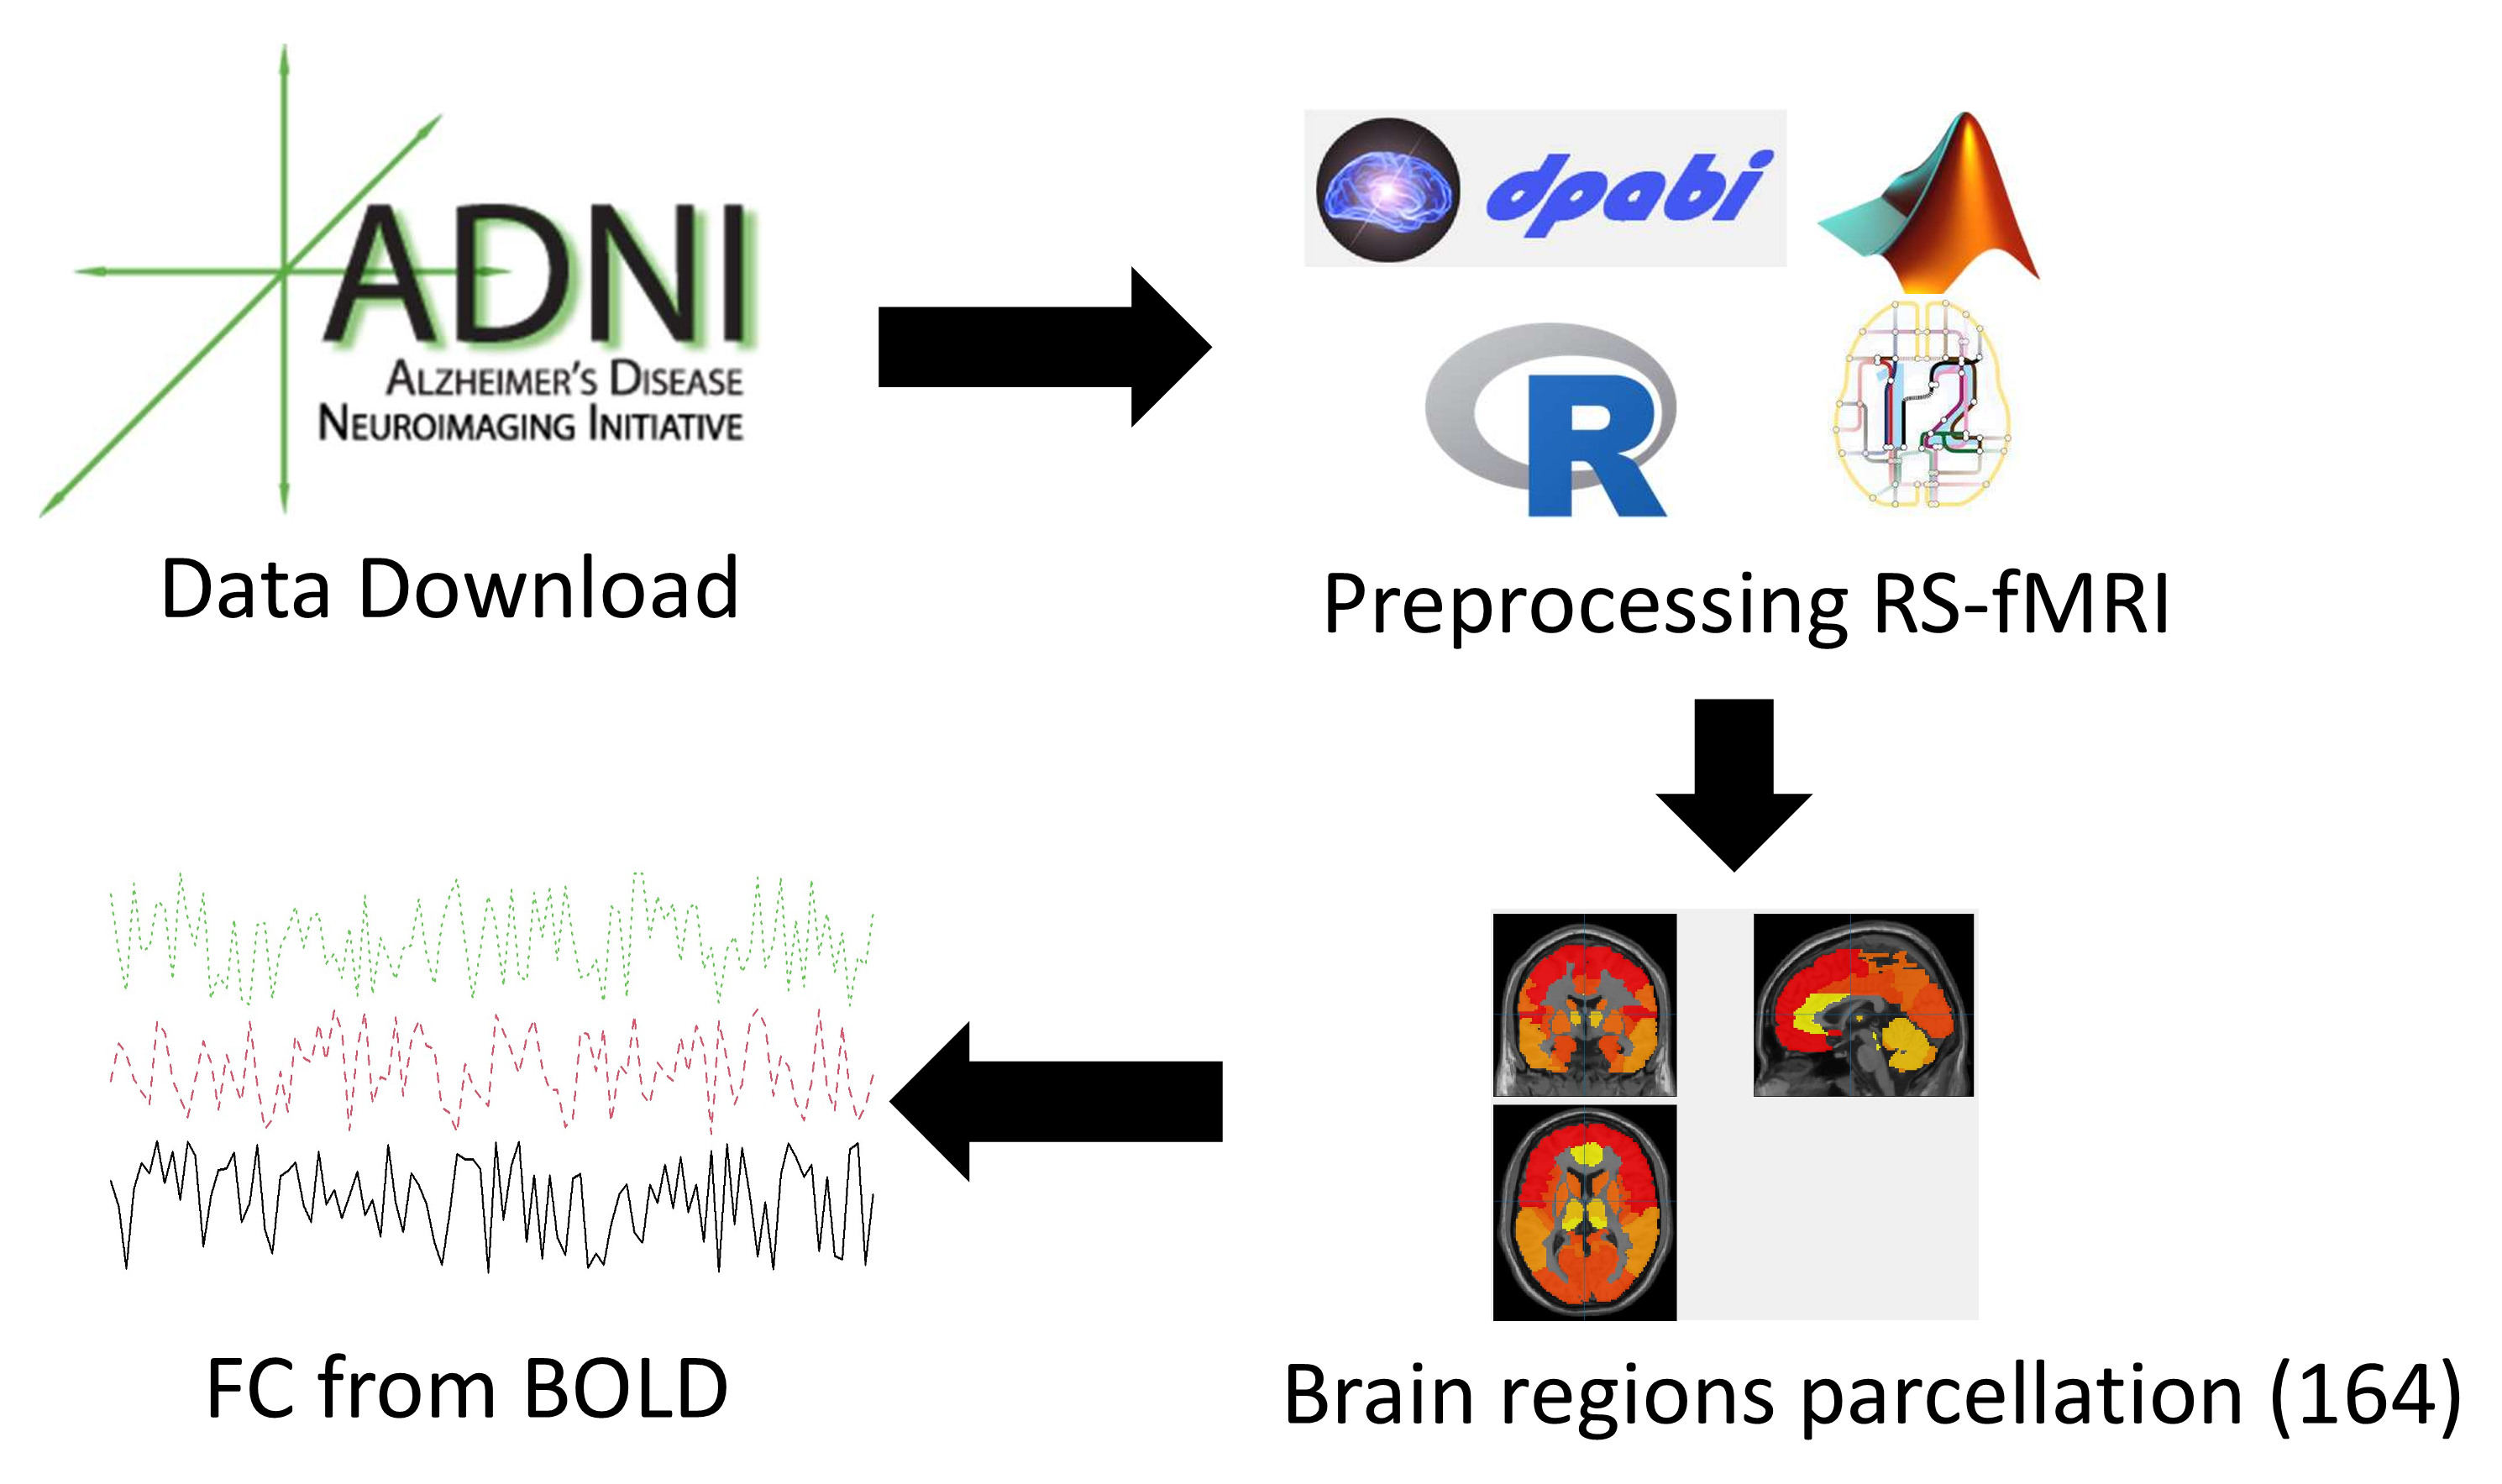
\includegraphics[width=\linewidth]{Figures/Preprocessing_4.png}
        \captionsetup{font=small} % 캡션의 글자 크기를 작게 설정
         \captionof{figure}{Preprocessing}
        \label{fig:image4}
    \end{minipage}
\end{figure}



    
%     \begin{figure}[ht]
%         \centering
%         \begin{minipage}{0.32\linewidth}
%             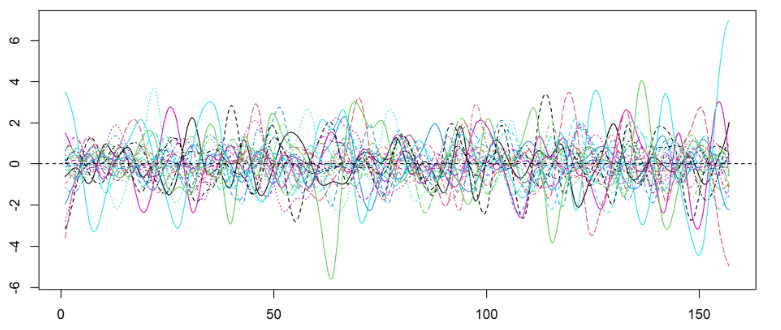
\includegraphics[width=\linewidth]{Figures/After_expansion.png}
%             \caption{Smoothed BOLD Signals}
%             \label{fig:image1}
%         \end{minipage}
%         \hfill
%         %=========================
%         \begin{minipage}{0.32\linewidth}
%             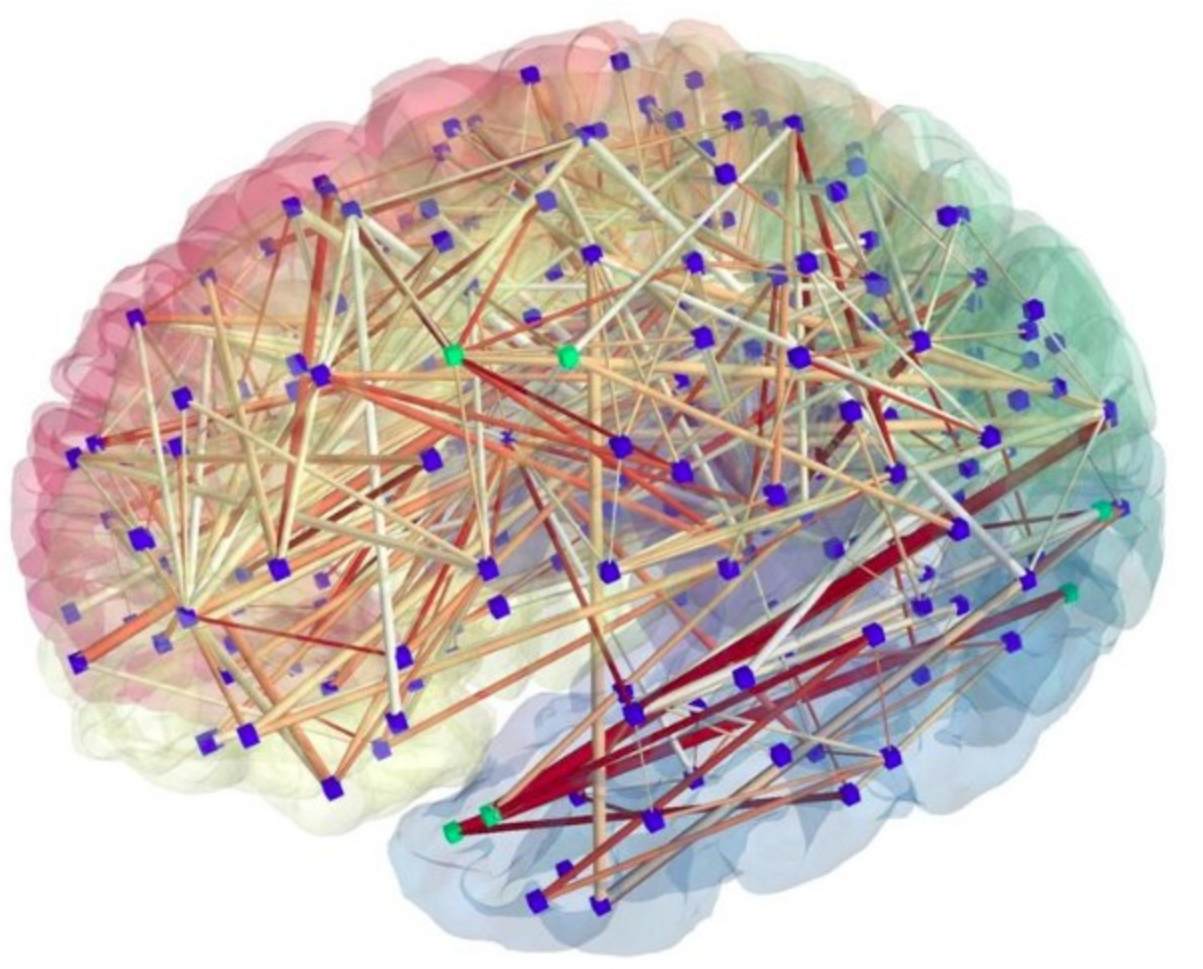
\includegraphics[width=\linewidth]{Figures/Functional Connectivity.png}
%             \caption{Functional Connectivity}
%             \label{fig:image2}
%         \end{minipage}
%         \hfill
%         %==========================
%         \begin{minipage}{0.32\linewidth}
%             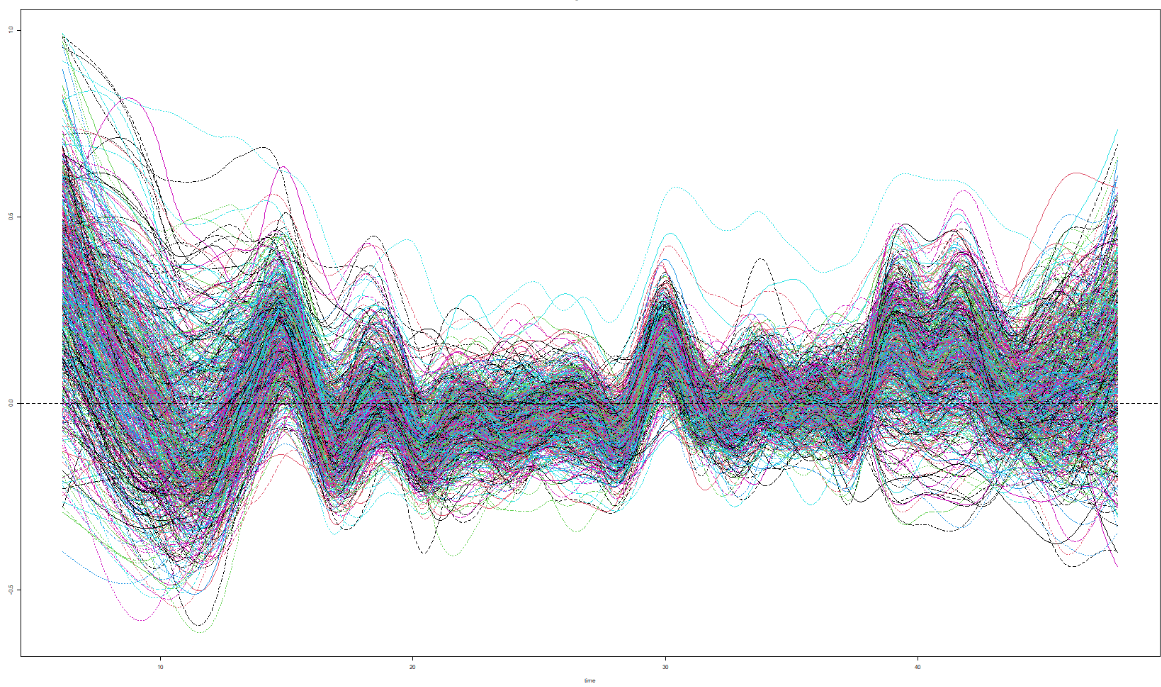
\includegraphics[width=\linewidth]{Figures/FC___FunImgARglobalCWSF___Smoothing.png}
%             \caption{Smoothed FC Signals}
%             \label{fig:image2}
%         \end{minipage}
%     \end{figure}

%     \begin{figure}[ht]
%   \centering
%   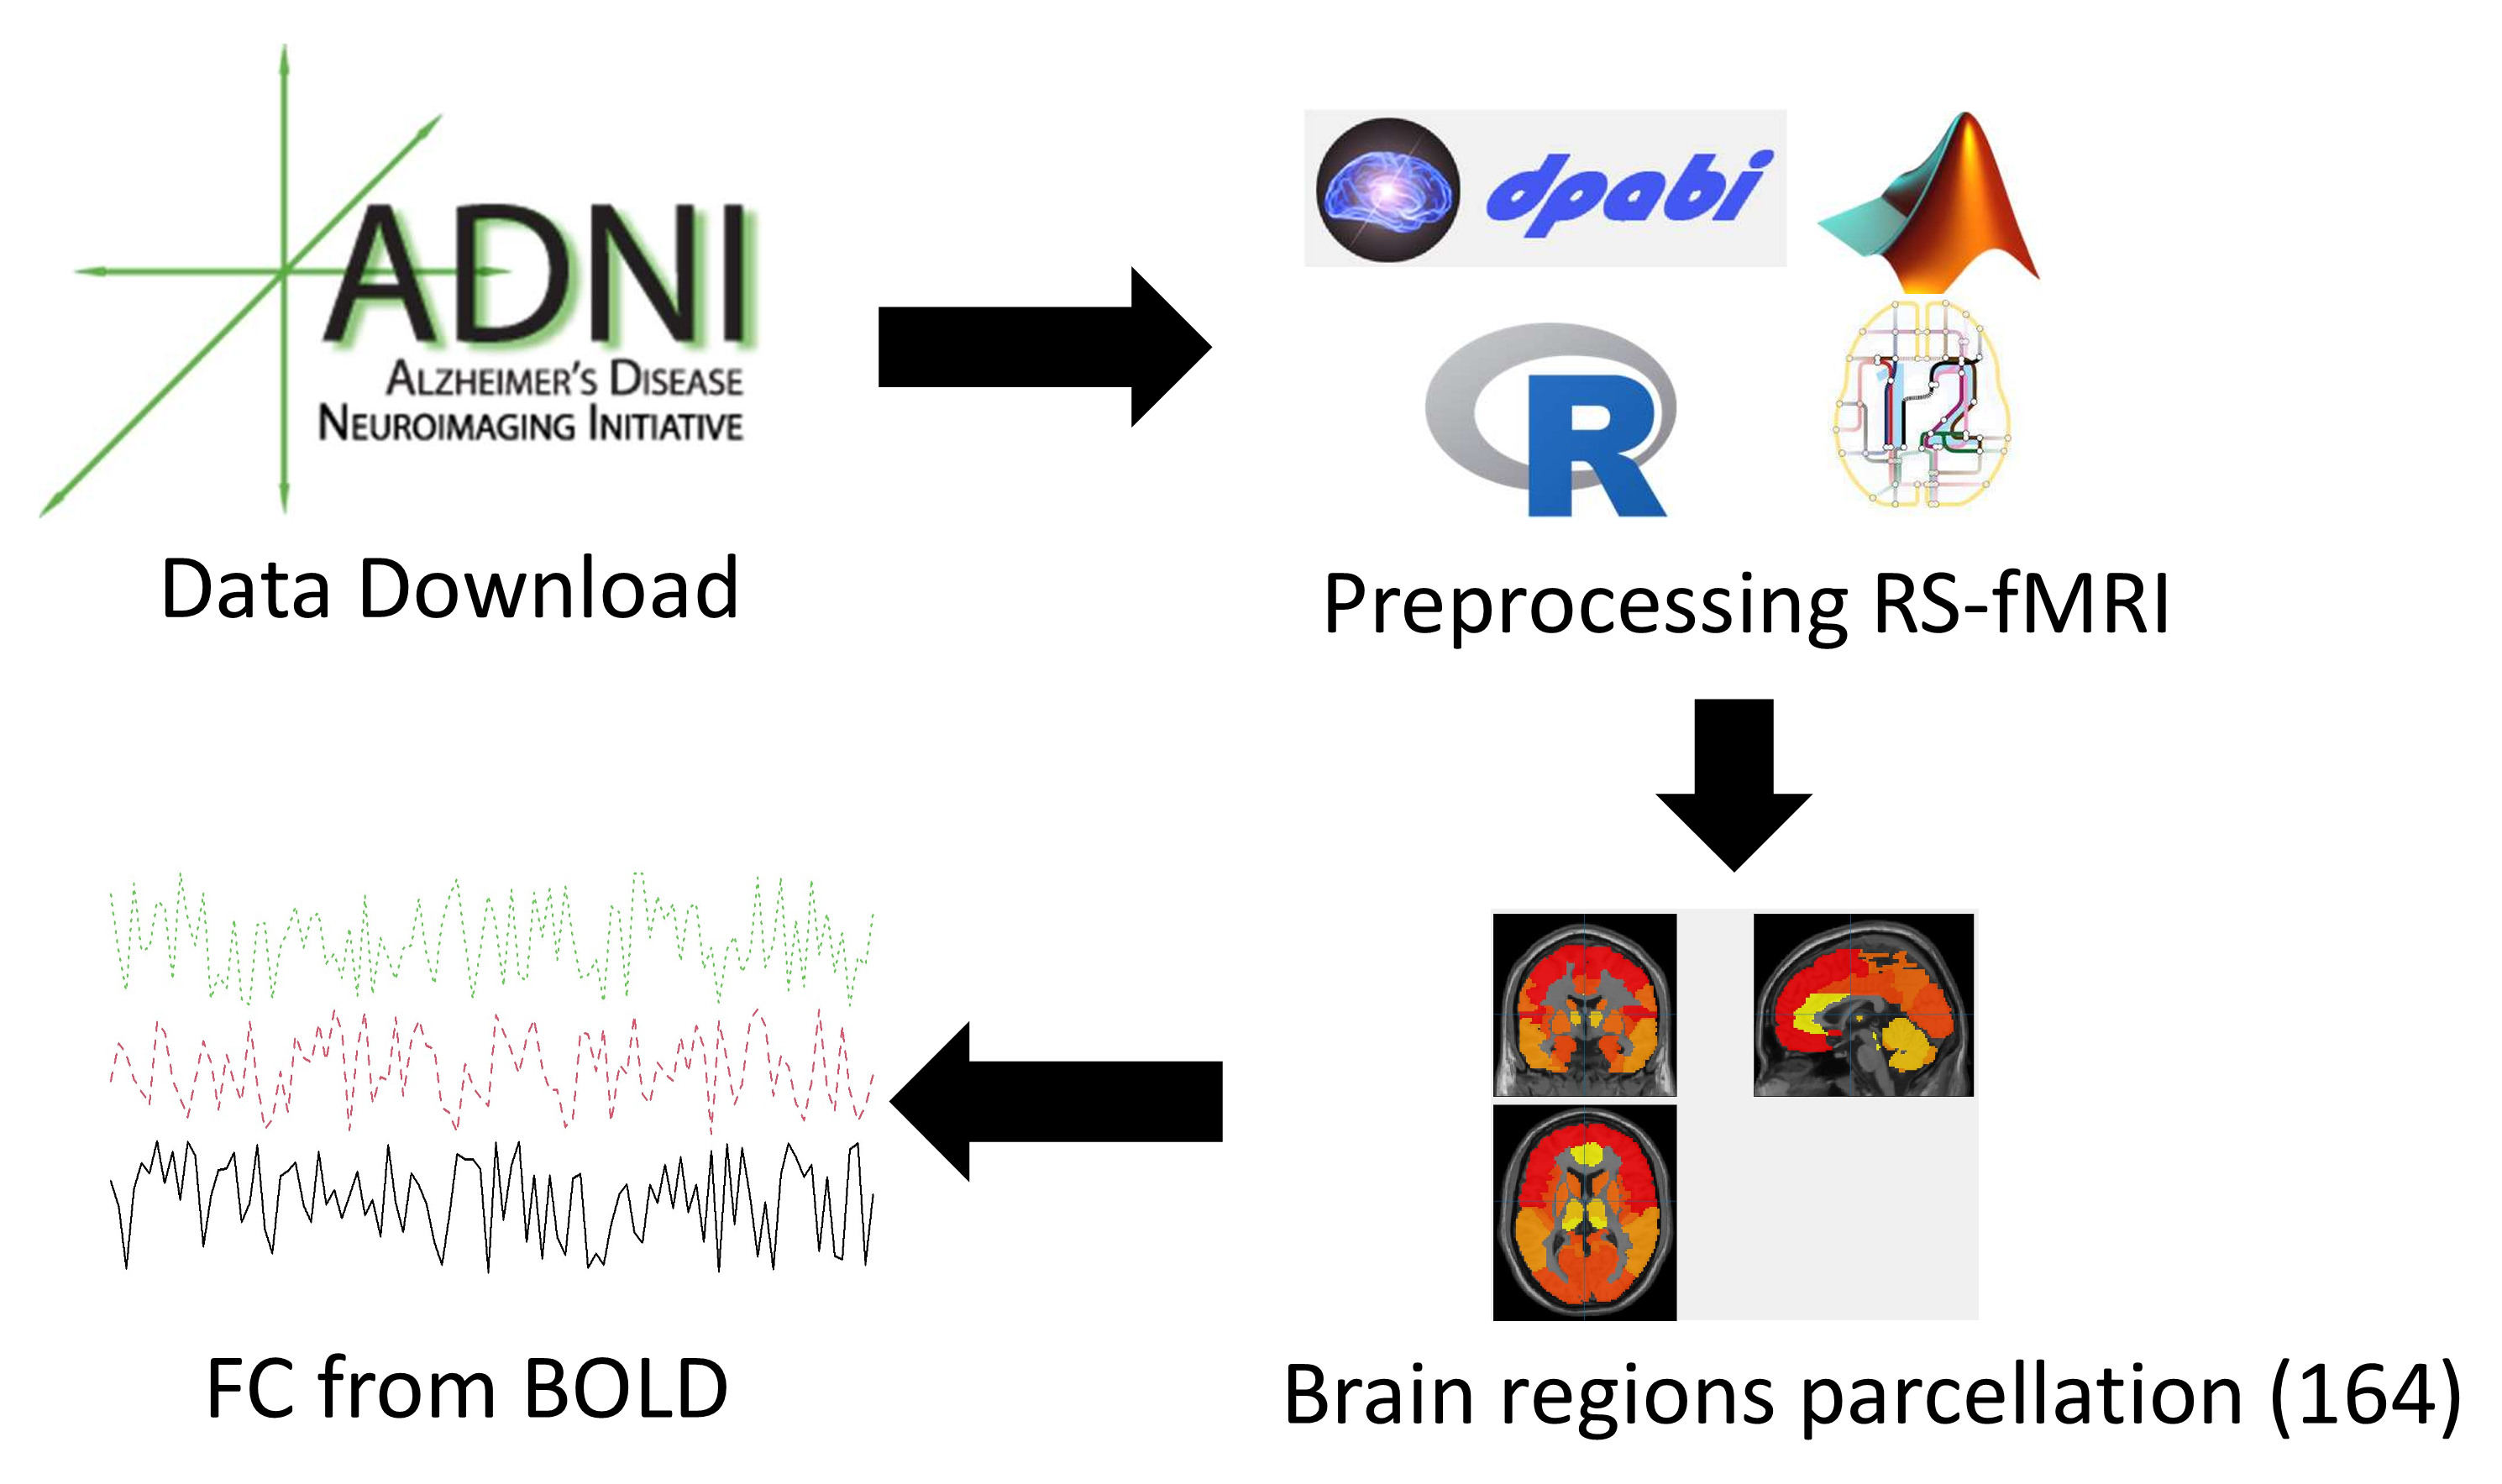
\includegraphics[width=0.5\linewidth]{Figures/Preprocessing_4.png}
%   \caption{Preprocessing}
%   \label{fig:myimage}
% \end{figure}

    
        \begin{itemize}
            \item Since it is difficult to capture internal variation among BOLD signals, it is difficult to apply functional PCA.

            \item From those BOLD signals, Functional Connectivity (FC) can be obtained by Pearson correlation.
        
            \item By brain distances, FCs can be sorted from one brain region, and this can be considered to be functional data.

            \item \textbf{B-spline basis expansion} can be applied to them.
            
        \end{itemize}
    
            \begin{equation*}
                f(t) \approx \sum_{j=1}^{J} c_j \phi_j(t)
            \end{equation*}

            \begin{itemize}
                \item \textbf{Functional PCA (FPCA)} was applied for each functional data from a brain region to extract features.
            \end{itemize}


     \begin{equation*}
         {{\rho }_{\xi }}\left( {{x}_{i}} \right)=\int{\xi \left( t \right){{x}_{i}}\left( t \right)dt}
     \end{equation*}


\columnbreak
%=======================================
% \section*{\tituloA{3.Preprocessing}}





%=======================================
\section*{\tituloA{3.Demographics}}

    \centering 


%         \begin{table}[ht]
% \centering
% \small % 폰트 크기 감소
% \begin{tabular}{lccc}
% \hline
% \textbf{Variable} & \multicolumn{3}{c}{\textbf{Summary}} \\ 
% \hline
% Diagnosis & CN & AD & \\
% & 295 (90\%) & 33 (10\%) & \\
% \hline
% Sex & \multicolumn{3}{c}{Male: 177 (54\%), Female: 151 (46\%)} \\
% \hline
% Handedness & \multicolumn{3}{c}{Right: 295 (90\%), Left: 33 (10\%)} \\
% \hline
% APOE4 & \multicolumn{3}{c}{0: 218 (67\%), 1: 96 (29\%), 2: 14 (4\%)} \\
% \hline
% Age & \multicolumn{3}{c}{74.36 \(\pm\) 7.64} \\
% \hline
% Education (y) & \multicolumn{3}{c}{16.75 \(\pm\) 2.41} \\
% \hline
% \end{tabular}
% \caption{Summary of demographic and clinical variables}
% \label{tab:variable_summary}
% \end{table}
\begin{table}[ht]
\centering
\scriptsize % 전체 테이블의 글자 크기를 줄임
\begin{tabular}{lccccc}
\hline
\textbf{Variable} & \multicolumn{5}{c}{\textbf{Summary}} \\ 
\hline
Diagnosis & CN: 295 (90\%) & & AD: 33 (10\%) & & \\
\hline
Sex & Male: 177 (54\%) & & Female: 151 (46\%) & & \\
\hline
Handedness & Right: 33 (10\%) & & Left: 295 (90\%) & & \\
\hline
APOE4 & 0: 218 (67\%) & & 1: 96 (29\%) & & 2: 14 (4\%) \\
\hline
Age & \multicolumn{5}{c}{74.36 \(\pm\) 7.64} \\
\hline
Education (y) & \multicolumn{5}{c}{16.75 \(\pm\) 2.41} \\
\hline
\end{tabular}
\label{tab:variable_summary}
\end{table}


% \begin{table}[ht]
% \centering
% \begin{tabular}{lccccc}
% \hline
% \textbf{Variable} & \multicolumn{5}{c}{\textbf{Summary}} \\ 
% \hline
% Diagnosis & CN: 295 (90\%) & & AD: 33 (10\%) & & \\
% \hline
% Sex & Male: 177 (54\%) & & Female: 151 (46\%) & & \\
% \hline
% Handedness & Right: 33 (10\%) & & Left: 295 (90\%) & & \\
% \hline
% APOE4 & 0: 218 (67\%) & & 1: 96 (29\%) & & 2: 14 (4\%) \\
% \hline
% Age & \multicolumn{5}{c}{74.36 \(\pm\) 7.64} \\
% \hline
% Education (y) & \multicolumn{5}{c}{16.75 \(\pm\) 2.41} \\
% \hline
% \end{tabular}
% \label{tab:variable_summary}
% \end{table}


% \begin{table}[ht]
% \centering
% \begin{tabular}{lccc}
% \hline
% \textbf{Variable} & \multicolumn{3}{c}{\textbf{Summary}} \\ 
% \hline
% Diagnosis & CN & AD & \\
% & 295 (90\%) & 33 (10\%) & \\
% \hline
% Sex & 0 & 1 & \\
% & 177 (54\%) & 151 (46\%) & \\
% \hline
% Handedness & 0 & 1 & \\
% & 33 (10\%) & 295 (90\%) & \\
% \hline
% APOE4 & 0 & 1 & 2 \\
% & 218 (67\%) & 96 (29\%) & 14 (4\%) \\
% \hline
% Age & \multicolumn{3}{c}{74.36 \(\pm\) 7.64} \\
% \hline
% Education (y) & \multicolumn{3}{c}{16.75 \(\pm\) 2.41} \\
% \hline
% \end{tabular}
% \label{tab:variable_summary}
% \end{table}
            
%=======================================
\section*{\tituloA{4.Classification Models}}
\begin{flushleft}
To take advantage of the \textbf{inherent group information} defined by ROIs, Group penalties were applied to logistic models.
\end{flushleft}

    \centering 
    \begin{itemize}
    \item \small Group LASSO: 
    \[ \lambda \sum_{g=1}^{G} \sqrt{p_g} \| \beta_g \|_2 \]
    \item \small Group Elastic-Net: 
    \[ \lambda \left( \alpha \sum_{g=1}^{G} \| \beta_g \|_1 + \frac{1-\alpha}{2} \sum_{g=1}^{G} \| \beta_g \|_2^2 \right) \]
    \item \small Group MCP (Minimax Concave Penalty): 
    \[ \sum_{g=1}^{G} \left( \rho(\| \beta_g \|_2; \lambda, \gamma) \right) \]
    \item \small Group SCAD (Smoothly Clipped Absolute Deviation): 
    \[ \sum_{g=1}^{G} \left( \phi(\| \beta_g \|_2; \lambda, a) \right) \]
\end{itemize}


%=======================================
\section*{\tituloA{5.Results}}
    \centering 
\begin{table}[ht]
\centering
\caption{AUC from logistic regression with group penalty using FPCA}
\label{tab:classification_group}
\begin{tabular}{|l|l|l|l|l|}
\hline
\textbf{Pipeline} & \textbf{Group Penalty} & \textbf{FPCA} & \textbf{FPCA+Demo} & \textbf{Demo} \\ \hline
\multirow{4}{*}{FunImgARCWSF} & Group Elastic-net & 0.49 & No Conv & 0.72 \\ \cline{2-5} 
 & Group LASSO & 0.68 & 0.70 & 0.72 \\ \cline{2-5} 
 & Group MCP & 0.64 & 0.62 & 0.72 \\ \cline{2-5} 
 & Group SCAD & 0.47 & 0.70 & 0.72 \\ \hline
\multirow{4}{*}{FunImgARglobalCWSF} & Group Elastic-net & No Conv& 0.72 & 0.72 \\ \cline{2-5} 
 & Group LASSO & \textbf{0.81} & \textbf{0.90} & 0.72 \\ \cline{2-5} 
 & Group MCP & 0.69 & 0.81 & 0.72 \\ \cline{2-5} 
 & Group SCAD & 0.73 & 0.83 & 0.72 \\ \hline
\end{tabular}
\end{table}


\begin{tabular}{|l|l|}
\hline
\textbf{Brain Region} & \textbf{Function} \\
\hline
Posterior Cingulate & Memory, attention \\
\hline
Cuneus & Visual processing \\
\hline
Fusiform Gyrus & Facial recognition \\
\hline
Paracentral Lobule & Motor/sensory processing \\
\hline
Temporal Pole, Mid Temporal & Language, emotion \\
\hline
\end{tabular}
    
%=======================================
% \section*{\tituloA{References}}
\begin{enumerate}
	\item[[1]]\small{SOBRENOME, Nome do autor (abreviado). Título do artigo. Título da Revista, (abreviado ou não) Local, Número do Volume, Número do Fascículo, Páginas inicial-final, mês e ano}
 \end{enumerate}



%=================================================
\section*{\tituloA{Acknowledgments}}

\begin{itemize}
    \item \scriptsize This material was based on work partially supported by the Institute of Information \& communications Technology Planning \& Evaluation(IITP) grant (No. 2020-0-01441, Artificial Intelligence Convergence Research Center(Chungnam National University))
    \item \scriptsize This work was also partially supported by the National Research Foundation of Korea(NRF) grant funded by the Korea government(MSIT) (No. NRF-2022M3J6A1084843, No. NRF-2021R1C1C1013936).
\end{itemize}






\end{multicols}

\end{document}
